\chapter{Analise de outros artigos}
\section{Calculo da informação de Fisher para sistemas complexos}
\subsection{Introdução}
\label{sec:Calculo do periodo}
A informação de fisher vem se provando uma otima metrica para estimativas e medições de sistemas complexos.
Como, por definição, ela nos diz o quão bem conseguimos estimar um parametro e de tabela tambem o grau
de desordem de um sistema, analisando ela para parametros e variaveis de um sistema ecologico, de
acordo com seu valor e suas variações, conseguimos estimar se um modelo está ou não entrando em
regime de transição e esta mudando de regime. Respondendo a uma pergunta, mudanças positivas da
informação de fisher indicam que o sistema está indo para um regime mais organizado e mudanças
negativas indicam que ele está indo para um regime mais desogarnizado. Mas uma coisa que era
necessaria, era ele ser ciclico e sabermos esse periodo. Claro que para modelos reais e complexos
isso muitas vezes não é possivel e muitas vezes se tinha um jogo de adivinhação e chute numerico
para que se estimasse o periodo. Em um outro artigo, que escreverei depois, eles propoem colocar um
valor inicial aleatorio, calcular a media da informação de fisher e sua variação sigma para um
periodo, depois ir ajustado o periodo até que variação tendesse a zero. Algumas hipoteses sistemas
foram feitas, conhecidas como Hipoteses dos sistemas sustentaveis
\begin{enumerate}\label{hip:Hipotese dos modelos sustentaveis}
    \item Para um regime sustentavel, a media da informação de fisher num periodo T tem de ser maior que
    zero e constante pelo periodo de tempo
    
    \item Quando o valor de Fisher aumenta o sistema esta ganhando informação, mudando de regime e
    aumentando sua ordem
    
    \item Quando o valor de Fisher diminui, o sistema esta perdendo informação, mundando de regime e
    diminuindo sua ordem
    
    \item O regime no qual o sistema está vai mudar se o valor de Fisher no periodo apresentar uma
    queda ou uma subida brusca na ordem dinamica. Como não foi feita nenhuma delimitação concreta
    sobre o que é uma queda ou subida brusca, um especialista vai definir isso.
\end{enumerate}
Enquanto o papel do artigo orginal é achar o periodo T, por hora não farei a discussão disso, por
motivos de não ser o foco princial inicialmente, mas ficara guardado e é interessante saber que
sendo relativamente recente, 2020, ainda se tem problemas e essa informação ainda é usada. Outro
ponto importante é que posteriormente ela usa a informação de fisher em sistemas que não sao
ecologicos no sentido natural, mas no sentido social e economico tambem, mostrando por exemplo, a
mudança de regime com o crescimento populacional, com o aumento de setores de energia, industrial, a
informação de fisher muda para mostrar essa mudança. Então é algo a se pensar
\section{Detecção e Avaliação de flips ecologicos usando informação de fisher (2008)}
\subsection{Introdução}
Como foi mencionado no primeiro artigo, o método de calculo, por mais que util, sofria de alguns
problemas e um deles era a extrema sensibilidade do calculo, em que qualquer barulho, erro na
estivativa do ciclo, ou falta de dados fazia com que a leitura do grafico ficasse um pouco
distorcida. Nesse artigo, ele tenta achar um novo jeito de calcular, ainda usando a informação de
fisher, mas de forma com que seja mais robusta e dê ainda mais informações, como a intensidade e a
propagação do flip ecologico. A propagação se diz em quantas variaveis observaveis essas mudanaças
estão afetando. Foi tambem nesse artigo que eles incrementam a Hipotese dos regimes sustentaveis ja
apresentada em sua forma moderna em \ref{hip:Hipotese dos modelos sustentaveis}. \par
\subsection{Desenvolvimento}
Uma das dificuldades dos calculos era obter as derivadas de ordem 2 dos datasets reais utlizados, pois
tinhamos dados com uma certa distancia entre si, o que dificultava essa medição. Como no artigo
original, eles lidaram, em sua maioria, com datasets com uma escala temporal de kAnos, uma
interpolação linear para que os dados fiquem regularmente espaçados e a média dos 3 pontos, essa
dificuldade foi circundada, tirando um pouco o erro e deixando a função mais suave. Mas nem sempre
isso sera possivel e no dataset do pacifico, com uma quantia grande de variaveis e uma escala
temporal pequena, a informação de fisher, por mais que calculada, ainda tinha problemas em sua
apresentação. Alem de que, não dava tempos exatos de quando ocorriam mudanças, mas mostrava que
ocorria a mudança de informação com a mudança de regime. Esse artigo tenta remediar isso, achando um
modelo mais robusto, que mostre quando ocorre essas mudanças. \par
A matematica para isso, eu vou deixar de lado por hora, pois não é necessaria para o momento atual. \par
A aplicação do modelo foi feita para um caso puramente matematico e depois para o caso do estreito
de bering. Para o modelo matematico, foi usado o modelo da eutrofização de um lago, onde se é
possivel alterar o nivel de barulho e quantidade de dados que temos ao longo do tempo. Para um
modelo com muitos dados e nenhum barulho e muitos dados e pouco barulho, se é claro a queda abrupta
de informação de fisher no ponto de mudança de regime. Para o caso com poucos dados e barulho, se vê
claramente a queda de fisher, mas ela ocorre por um periodo maior, não sendo o pico exato dos outros
dados.
\begin{figure}[H]
    \centering
    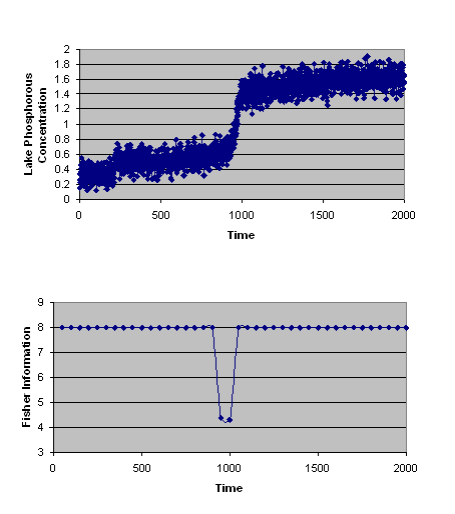
\includegraphics[width=0.8\textwidth]{fihser mts dados pouco barulho.png}
    \caption{Eutrofização de um lago com pouco barulho}
    \label{fig:Eutrofizacao de um lago com pouco barulho}
\end{figure}
\begin{figure}[H]
    \centering
    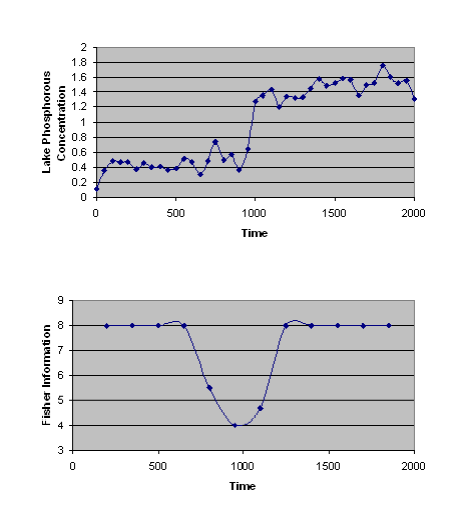
\includegraphics[width=0.8\textwidth]{fisher poucos dados baruhlo.png}
    \caption{Eutrofização de um lago com muito barulho}
    \label{fig:Eutrofizacao de um lago com muito barulho}
\end{figure}
\subsection{Conclusão}
Para o conjunto de dados reais, do estreito de bering, usaram-se 65 variaveis e fizeram a separação
entre as ambientais e as animais. Enquanto os dados são relativamente espaçados, medidos anualmente
e com muito baruhlo, ainda é possivel ver a mudança de informação de fisher, não sendo o pico
abrupto mais sim uma area de minimo  e o começo de uma queda para um flip mais recente. Não é
possivel necessariamente definir exatamente o ano do flip, talvez pelo método de calculo dele, que
foi por uma especie de convolução, mas se é possivel atribuir um intervalo a qual se tem o minimo e
atribuir o flip la. Enquanto sim é mais robusto, não precisou saber o momento exato do flip, coisa
que no artigo original eles precisavam, foi se calculado com um dataset barulhento e real de forma
bastante satisfatoria. O nivel de propagação pode ser visto mudando o nivel de restrição no calculo
(parte matematica não escrita ainda). Uma grande propagação é vista como uma queda abrupta na
informação de fisher para conjuntos de restrição baixa. Ademais, a maior queda observada no regime
de 77 do que de 89 nos diz que o de 77 foi de maior magnitude e possivelmente de maior impacto no
ecosistema. O nivel de restrição é algo que não é definido quanto para cada, depende um pouco de
teste para identificar. Uma restrição muito baixa e não vamos detectar nenhum regime, e uma muito
alta tambem não vmaos identificar. A depender do nivel de restrição tambem, não conseguimos detectar
flips de menor propagação, o que pode ser problematico.
\section{Identificações em shifts ecologicos (2008)}
\subsection{Introdução}
Enquanto tem sido um grande topico de estudos e interesse da comunidade cientifica entender, tentar
prever, identificar e analisar as mudanças de regimes ecologicos que ocorrem, interessantemente a
aplicação da estatistica não foi muito usada, apenas iniciando-se relativamente recentemente, mas
ainda extremamente restrito e muitas vezes usados em apenas certas ocasiões e muitas vezes apenas em
ecossistemas marinhos. Mas com o grande desenvolvimento da estatistica, da area de Teoria da
informação, vem se tornando cada vez mais viavel essa utilização e esse artigo visa reunir e
apresentar os principais métodos que se tinham desenvolvidos na epoca (2008), alem de mostrar suas
vantagens, problemas e possiveis coisas a serem optimizadas. \par

Em um modelo muito simplificado de ecologia, em um sistema vamos supor 2 estados, independente de
que sejam estaveis, lineares, ciclicos, caoticos, mas a mudança abrupta entre esses dois estados, ou
seja, indo do 1 para o 2 ou do 2 para o 1 identificam um shift ecologico. O grande uso da
estatistica e da matematica, sendo justo, é a identficação desses picos. Se fossemos colocar um
pulo, entre um estado ao outro, supondo, uma das coisas mais importantes na estatica de inferencia
foi a detecção desses pulos em um conjunto de dados.

\subsection{Métodos de detecção}
\begin{enumerate}
    \item O primeiro a ser considerado é apenas um tratamento e uma analise preliminar dos dados. A
    ideia principal é tentar resaltar esses pulos entre os dados para que uma analise mais simples
    consiga detectar esses flips. Um dos métodos mais usados, que é simples, facil e relativamente
    util, mas tem problemas que serão colocados depois é simplesmente achar o desvio padrão dos
    dados e fazer uma analise sobre (perguntar a mari posteriormente sobre). Esse método, simples,
    porem pode levar a falsos positivos, o que não é o desejado.
    
    \item Um outro método que é bastante utilizado, inclusive no dataset do estreito de bering, é a
    analise das componentes principais (PCA). Enquanto muito util e relativamente eficaz, detectando
    sim o shift, ela possui erros. Ela naturalmente é linear, pois acha os versores que maximizam a
    variancia do dataset, não capturando relações não lineares. Alem de que, em um sentido de
    Algebra linear, pode e vão ocorrer distorções, variando de set a set, dos dados, pois um dos
    requerimentos é a independencia linear. Alem disso, ela pode mostrar multimodalidade em datasets
    que não são, inclusive podendo apresentar para dados retirados de uma normal. enquanto util e
    bom para vizualização de dados, não é a mais certeira e eficaz
    
    \item Um método que pode ser usado é um teste de hipotese. Mais especifico, usando um método de
    intervenção pode ser usado. Mas por que colocar um teste de hipotese? Dados reais apresentam um
    alto grau de barulho, então métodos que olham para valores extremos, por exemplo, podem detectar
    um falso postivo. Com um teste de hipotese, colocando um nivel de confiança \(\alpha =5\% \),
    podemos evitar um pouco esses falsos positivos. Um dos problemas de usarmos o método de
    intervenção é que precisamos, necessariamente, saber o tempo em que ocorreu a mudança, o que
    implica estimarmos usando algum outro método. Podemos fazer um teste para cada ponto para
    sabermos se houve ou não uma mudança de regime, obtendo valores criticos, que devem ser mais
    altos que na estatistica classica. (esse finalment eu não entendi, perguntar para a mari dps.)
\end{enumerate}
\subsection{Conclusão}
Existem diversas outras formas de se explicar e mostrar as mudanças ecologicas, não so com a
informação de fisher. Algumas, não tão complexas como as outras, mas todas apresentando algum ponto
negativo sobre. A grande questão que analisei é a incerteza quanto ao tempo exato de se identificar
a mudança, sendo ela extremamente significativa ou não. Alem de que, muitas vezes se requerem muitas
variaveis e uma computação talvez um pouco intensa e complexa, então é algo a sem pensar. Num lado
mais de aprensentação, talvez uma analise visual e tentar mostrar a estatistica seja algo
interessante, já que muitos não apresentam isso.
\section{Calculando e interpretando a informação de Fisher. Um estudo de caso (2009)}
\subsection{Introdução}
Alem de seu uso na ecologia, esse artigo tambem cita o desenvolvimento da informação de fisher em
outras disciplinas, como economia, medindo a informação em uma pseudo-economia, sistemas urbanos e
ecossistemas regionais. (pesquisar mais sobre depois). Alem disso, como eu ja tinha pensado sobre,
se mostra ainda um pouco de dificuldadede no calculo da integral, necessitando de calculo, ou
estimativas, das derivadas de primeira e segunda ordem, que por si so já são trabalhosas, mas são
amplificadas pelo fato de os dados serem espaçados e com muito barulho. Alem de que ainda é de
dificil interpretação o valor que sai lá. O que extamente diz? Sua ordem de grandeza significa algo?
\subsection{Desenvolvimento, resultados e discussões.}
A solução analitica da equação de fisher é dado por
\begin{equation}
    I(t_i)=\frac{1}{T}\int_{t_i}^{t_{i+T}} \frac{(s^{\prime\prime})^{2} }{(s^\prime)^4 }
\end{equation}
onde
\begin{equation}
    s^\prime (t)=\sqrt{\sum_{i}^m(\frac{\mathrm{d}y_i}{\mathrm{d}t} )^{2} } 
\end{equation}
\begin{equation}
    s^{\prime\prime}(t)=\frac{1}{s^\prime }\sum_{i}^m\frac{\mathrm{d}y_i}{\mathrm{d}t} \frac{\mathrm{d}^{2} y_i}{\mathrm{d}t^{2}}
\end{equation}
Para casos de uma função quadratica, teriamos uma informação que vai para o infinito no seu ponto de
inflexão. Uma linear não nos da uma informação nenhuma e uma constante nos da uma informação
constante, assim como uma senoidal. Uma exponencial nos da uma informação exponencial inversa ao
valor da função. Se a exponencial da função cresce, a informação descresce e vice versa. O
interessante é a questão da periodica, pois nela, se tivermos o periodo \(T\) sua informação é
constante por todo periodo, então para uma analise ecologica o ideal é achar o periodo, pois
facilita a interpretação. Esse periodo pode ser estimado pelos métodos descritos em \ref{sec:Calculo
do periodo}. \par

A interpretação da informação pode vir direta das hipoteses citadas em \ref{hip:Hipotese dos modelos
sustentaveis}, onde se divermos sistemas em que \(\frac{\mathrm{d}I}{\mathrm{d}t} \approx 0\), eles
são considerados sustentaveis. Uma periodica, ou constante são teoricamente sustentaveis
de acordo com nossas hipoteses. Uma reta por sua vez, mesmto tendo uma baixa variação de fisher
não seria considerada sustentavel pois em qualquer instante que se mede ela, ela esta em um estado
diferente, por isso não seria sustentavel. Uma exponencial, sempre estando variando, indica um
sistema que ainda não se estabilozou e busca essa estabilidade. \par

Mesmo que um sistema seja estavel, muitas vezes ele pode estar em um estado que não interessa para
gente. Um lugar completamente deserto, onde praticamente nada vive é, em tese, sustentavel, pois a
variação da informação de fisher tende a zero. Mas é algo desejavel para nos? Tudo está na
interpretação e as vezes não necessariamente é algo completamente indesejavel perder informação de
fisher, desde que essa perca nos leve a algo que seja ecologico. O grande jogo esta na analise da
derivada da informação. \par

Fazer depois